\documentclass{beamer}
\usepackage[utf8]{inputenc}
\usepackage[T1]{fontenc}
\usepackage[english]{babel}
\usepackage[babel=true]{csquotes}
\usepackage{graphicx}
\usepackage[export]{adjustbox}
\usepackage{amsmath}
\usepackage{algorithm2e}
\usepackage{hyperref}
\usepackage{listings}
\usepackage[toc,page]{appendix}
\usepackage[backend=biber,style=alphabetic]{biblatex}


\graphicspath{ {../images/} }
\usetheme{Copenhagen}
\setbeamertemplate{page number in head/foot}[totalframenumber]


\title{Profile-guided optimization}
\subtitle{Speeding up LHCb software through compilation optimization}
\author{Oscar Buon}


\begin{document}

\begin{frame}
    \centering
    \begin{minipage}{0.2\textwidth}
        
\includegraphics[width=\textwidth]{logo_ISIMA_INP.png}
    \end{minipage}\hfill
    \begin{minipage}{0.2\textwidth}
        
\includegraphics[width=\textwidth]{logo_CERN.png}
    \end{minipage}\hfill
    \begin{minipage}{0.2\textwidth}
        
\includegraphics[width=\textwidth]{logo_LHCb.png}
    \end{minipage}

    \maketitle

    Supervisor: Sebastien Ponce
\end{frame}

\part{Introduction}
\section*{Introduction}
\part{Body}

    \begin{frame}
        \frametitle{CERN}

        Intergovernmental particle physics on France-Switzerland border.

        About  15,000 people working at CERN.

        Made discoveries that led to Nobel Prizes.

        World Wide Web was invented at CERN.
    \end{frame}

    \begin{frame}
        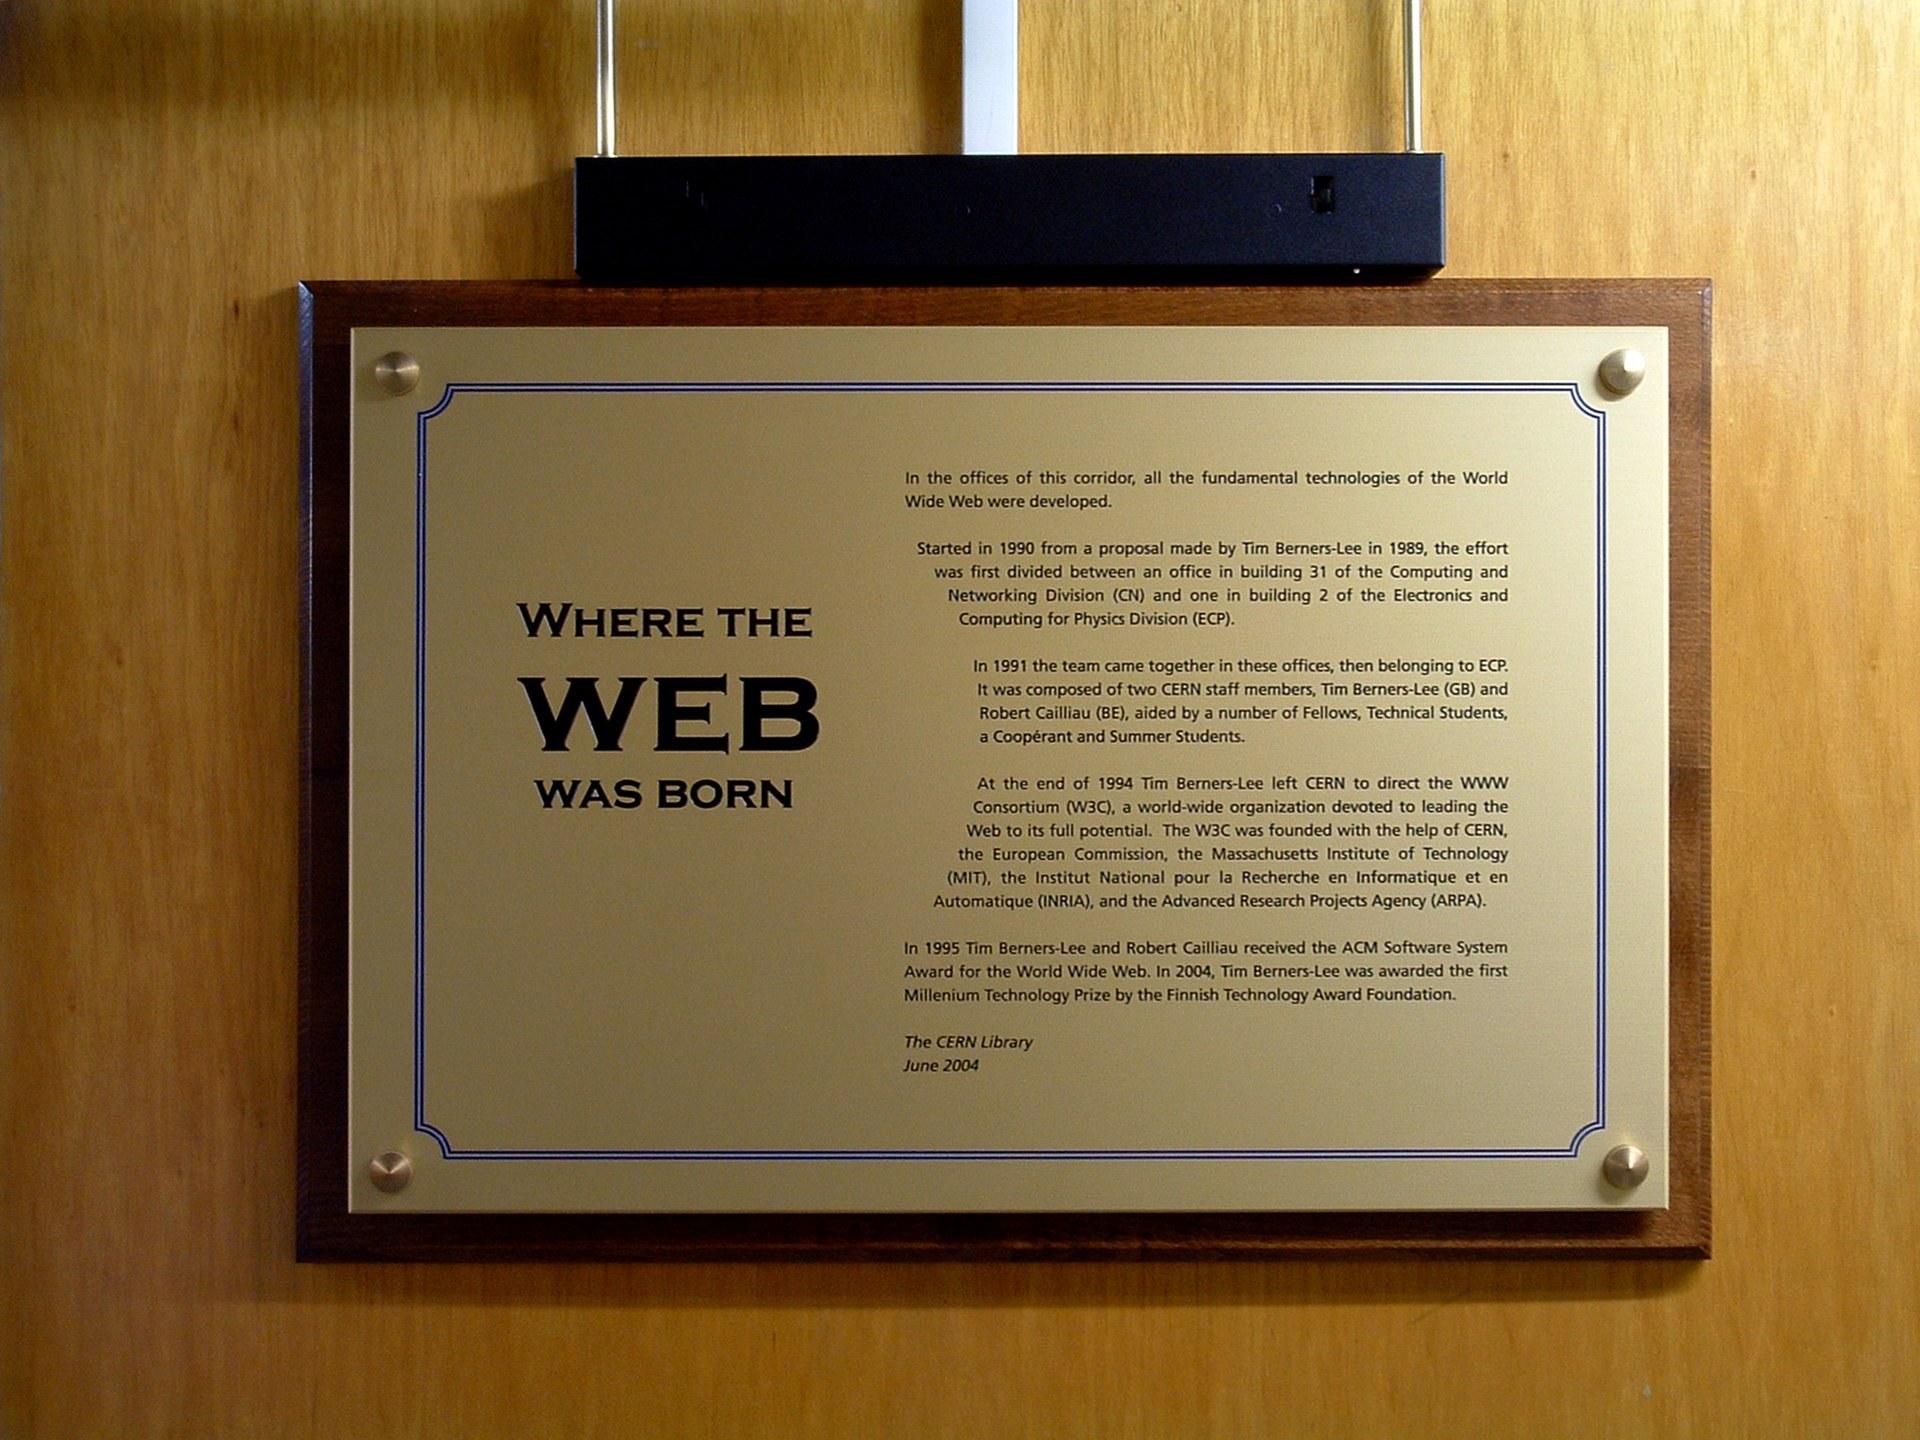
\includegraphics[width=0.75\textwidth]{WEB.jpg}
    \end{frame}

    \begin{frame}
        \frametitle{Large Hadron Collider (LHC)}

        \begin{itemize}
            \item Large Hadron Collider: particle collider
            \item $ 27 km $ (biggest in the world)
            \item $ \sim 100 m $ underground
        \end{itemize}

        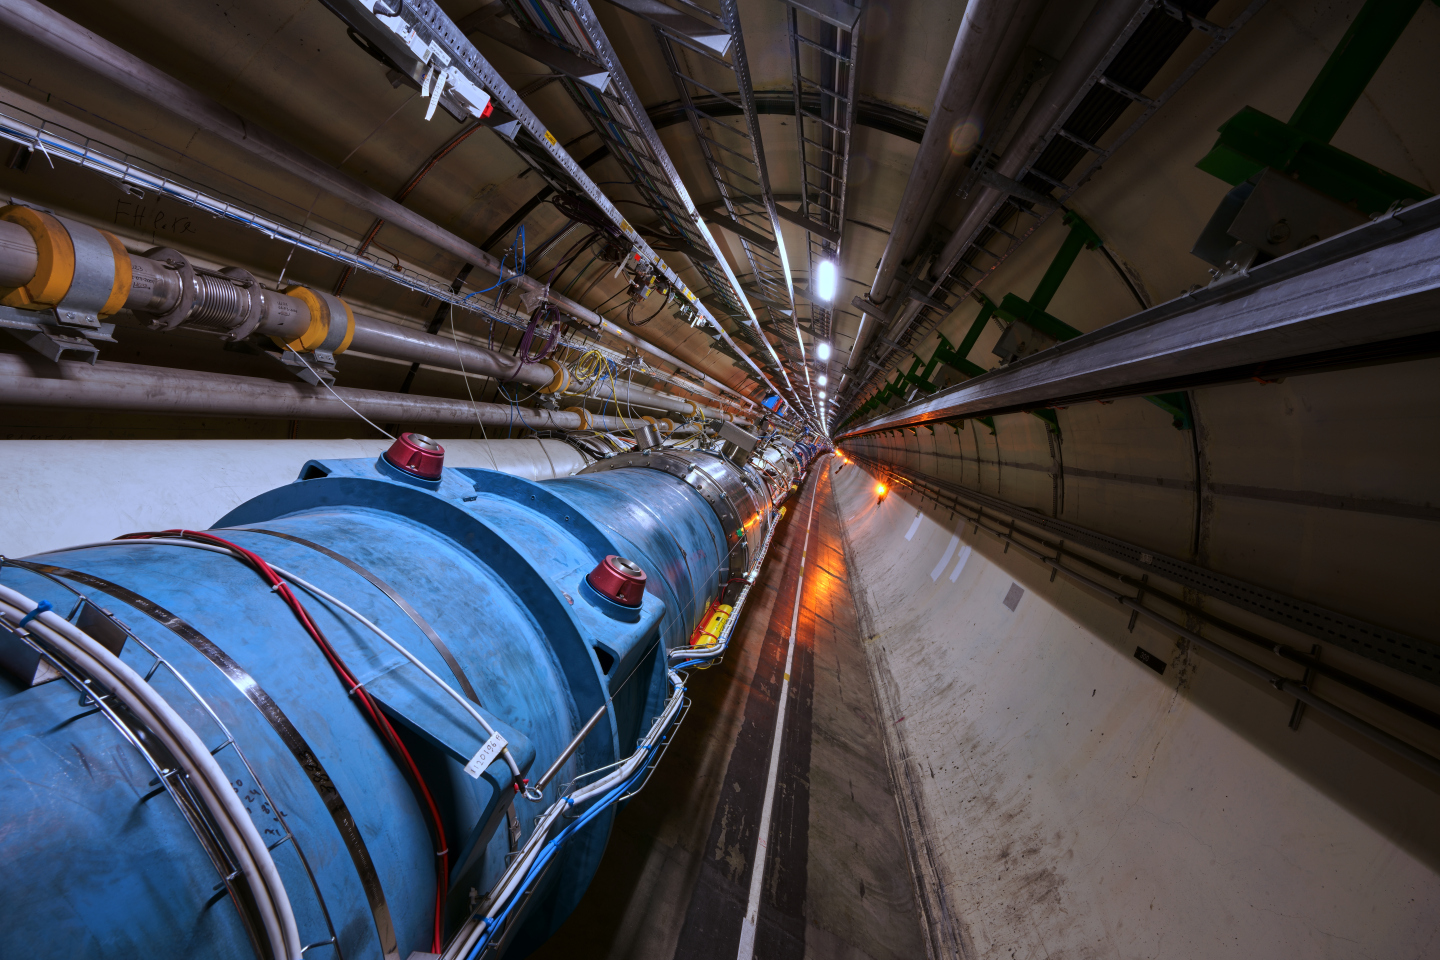
\includegraphics[width=0.5\textwidth]{LHC.jpg}
    \end{frame}

    \begin{frame}
        \frametitle{LHCb}

        \begin{itemize}
            \item One of the 4 main experiments installed on the LHC.
            \item More than 1,200 people working for the collaboration.
            \item Studies asymmetry between matter and antimatter via b-physics.
            Collision of hadrons (heavy particles).
        \end{itemize}

        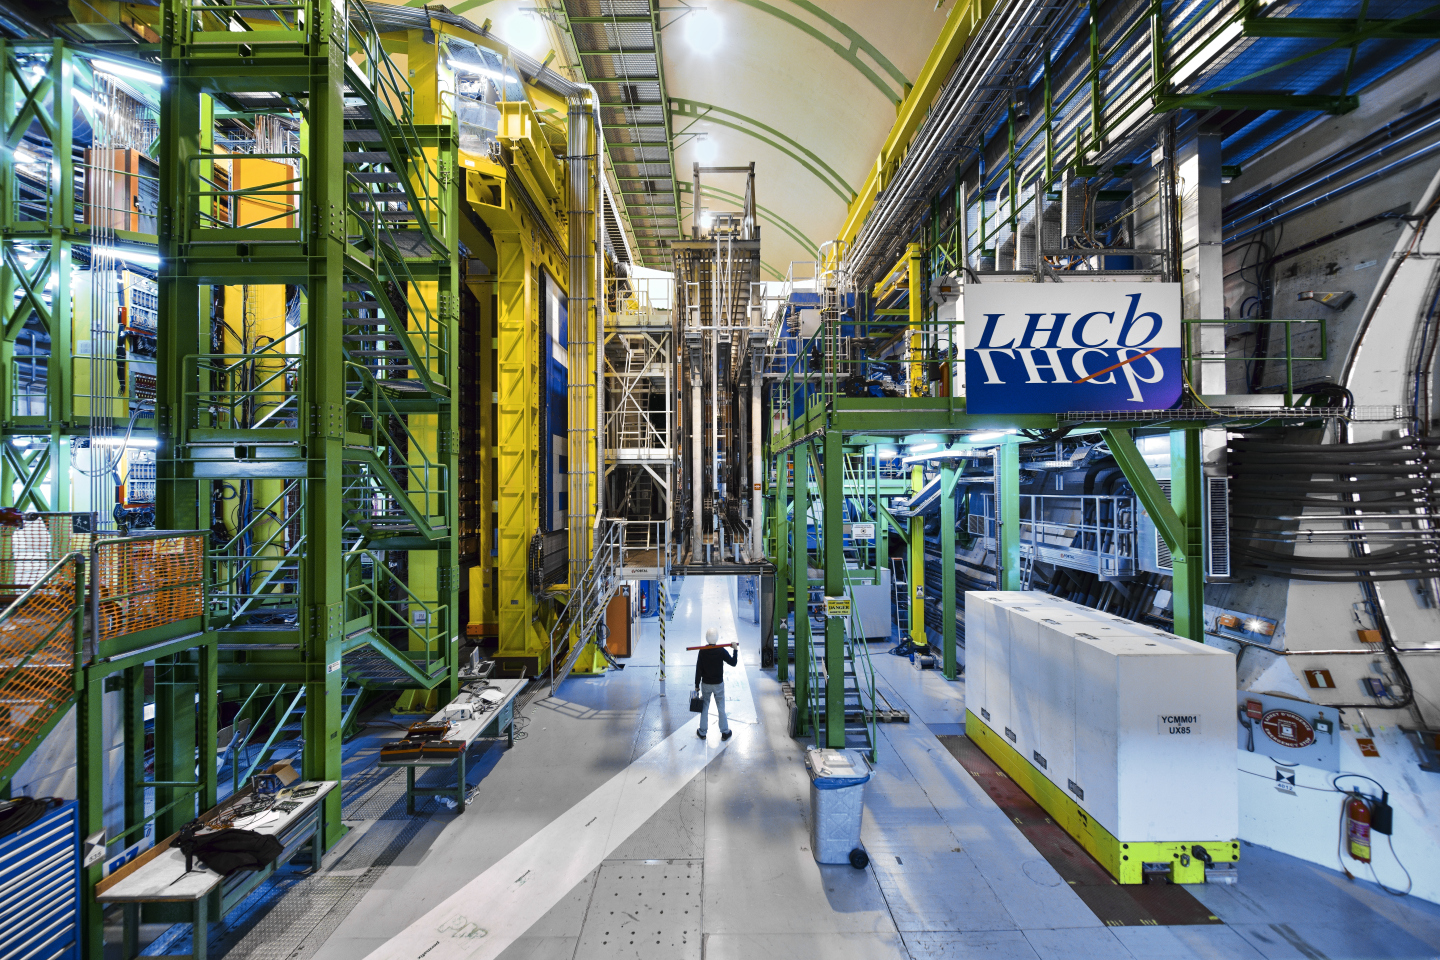
\includegraphics[width=0.5\textwidth]{LHCb.jpg}
    \end{frame}

    \begin{frame}
        \frametitle{Physics Computing}

        Important computing infrastructure.

        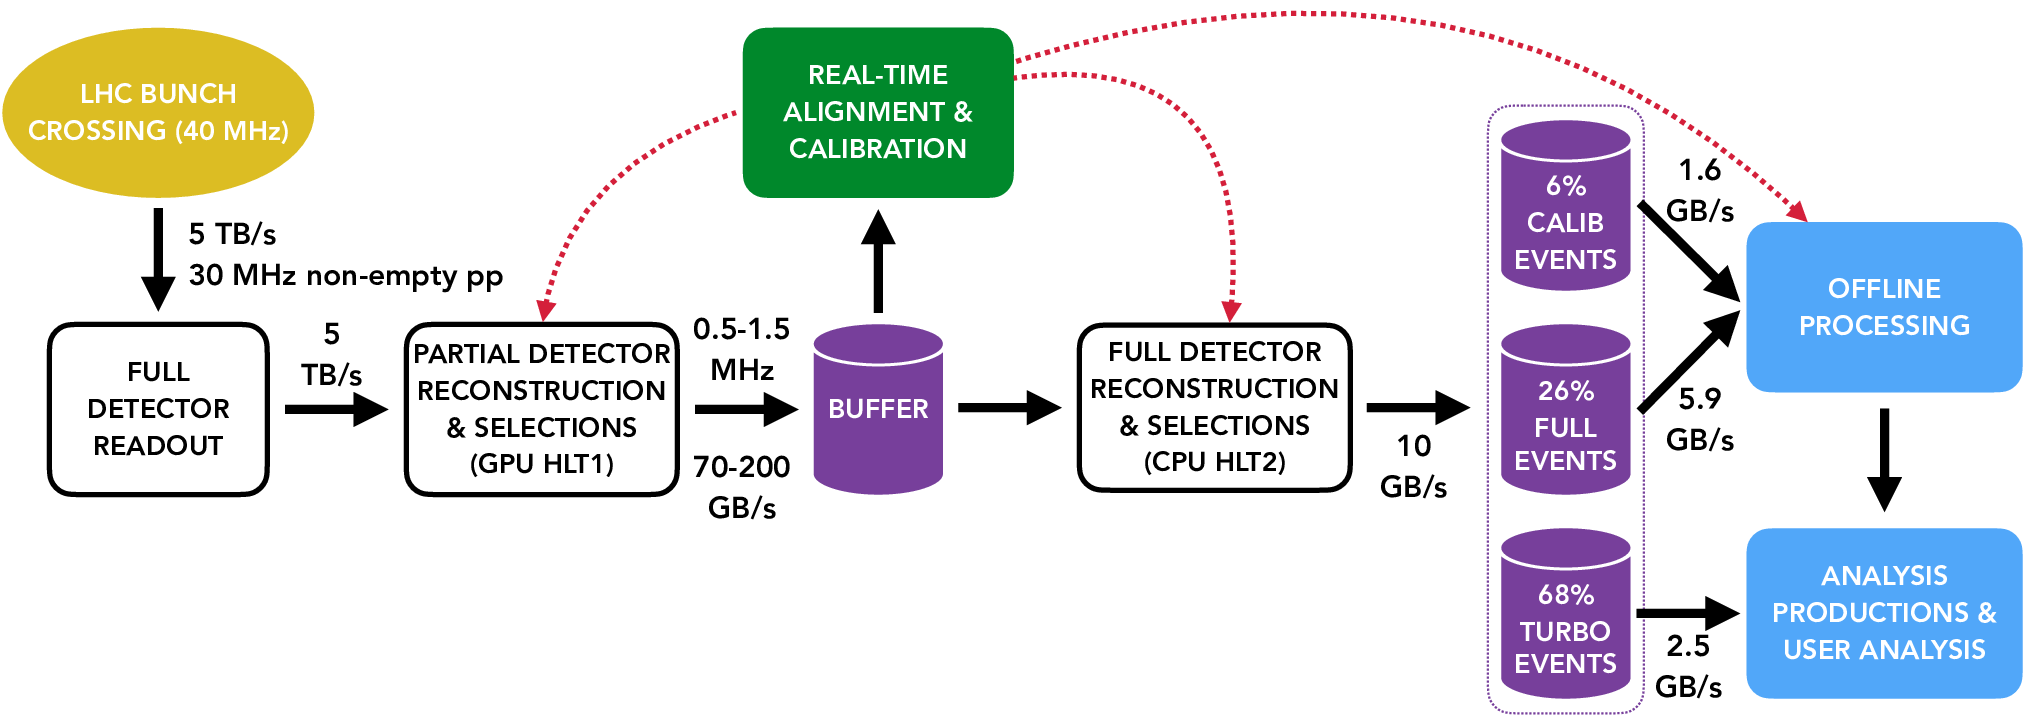
\includegraphics[width=\textwidth]{LHCb_stack.png}
    \end{frame}

    \begin{frame}
        \frametitle{Computing group}

        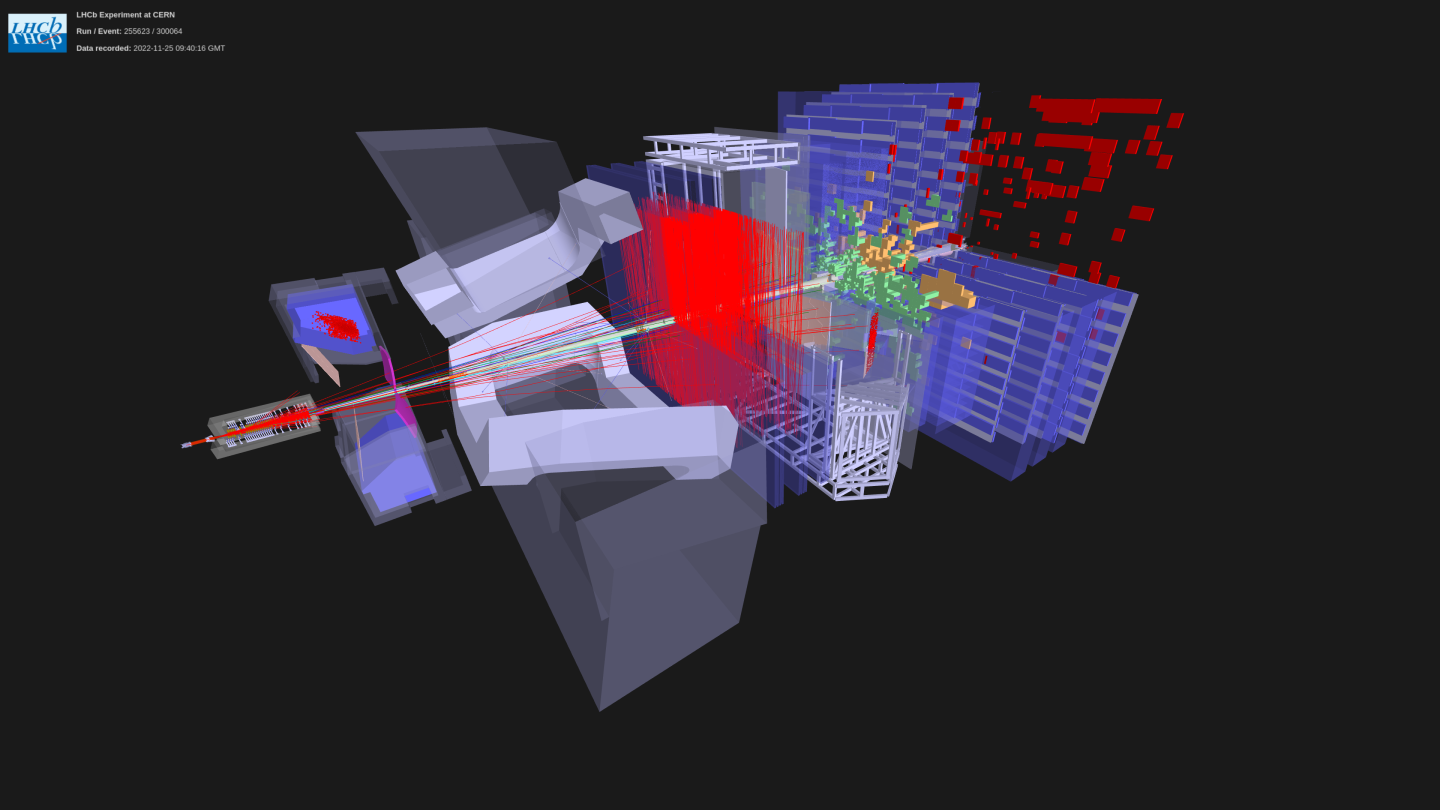
\includegraphics[width=0.75\textwidth]{LHCb_3D.png}

        The computing group has to maintain this infrastructure for LHCb.
    \end{frame}

    \begin{frame}
        \frametitle{Software}

        The software is a stack of programms:

        \begin{itemize}
            \item Common base shared with other experiments.
            \item LHCb specific programms.
            \item Reconstruction, simultation...
        \end{itemize}

        Millions lines of code which some are 30 years old.
        Code mainly written by non-software engineers.

        All of this is running on thousands of multithreaded Linux servers.
    \end{frame}

    \begin{frame}
        \frametitle{Table of contents}
        \tableofcontents
    \end{frame}

\section{Graphviz for printing graphs}

    \begin{frame}
        \tableofcontents[currentsection]
    \end{frame}

    \begin{frame}[fragile]
        \frametitle{Graphviz for printing graphs}

        Printing graphs was usefull to have an idea of the dependencies.

        Graphviz in CMake to create dependency graphs:
        \begin{itemize}
            \item CMake arg: \verb'--graphviz=path/to/files.dot'
            \item Convert to SVG: \verb'dot -Tsvg -o path/to/file.svg path/to/file.dot'
            \item Make arg: \verb'CMAKEFLAGS="--graphviz=path/to/files.dot"'
            \item Setting \verb'GRAPHVIZ_EXTERNAL_LIBS' to \verb'FALSE' is usefull.
        \end{itemize}

    \end{frame}

    \begin{frame}
        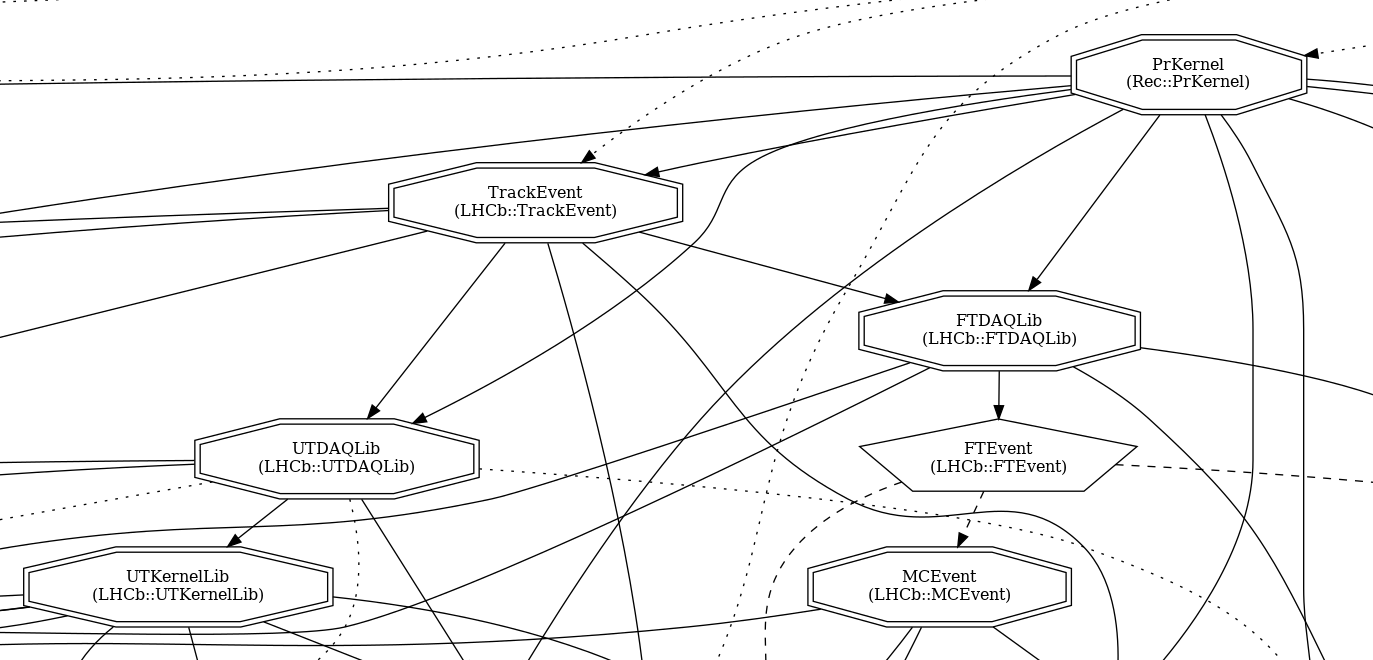
\includegraphics[width=\textwidth]{graphviz_cropped.png}
    \end{frame}

\section{Static libraries and modules}

    \begin{frame}
        \tableofcontents[currentsection]
    \end{frame}

    \subsection{Library types}

    \begin{frame}[fragile]
        \frametitle{Library types}

        \begin{itemize}
            \item STATIC: archive of object files that are merged to the executable at link time.
            \item SHARED: .so (Linux) file that is automatically linked to the executable at runtime (when starting it).
            Allows several executables to link with a library installed on the system.
            \item MODULE: same as shared but the module is loaded on demand via the \verb'dlopen' function, so not automatically.
        \end{itemize}
    \end{frame}

    \subsection{Static libraries}

    \begin{frame}[fragile]
        \frametitle{Gaudi Static libraries}

        \begin{itemize}
            \item Gaudi based on CMake.
            \item Created new Gaudi function for static libraries:
            \begin{itemize}
                \item Adapting the shared one.
                \item \verb'gaudi_add_library' $\Rightarrow$ \verb'gaudi_add_static_library'
                \item Replacing \verb'SHARED' by \verb'STATIC' in \verb'add_library' function call.
            \end{itemize}
        \end{itemize}
    \end{frame}

    \subsection{Static modules}

    \begin{frame}[fragile]
        \frametitle{Static modules}

        Linking modules as static libraries requires:
        \begin{itemize}
            \item \verb'-Wl,--whole-archive'
            \begin{itemize}
                \item without the linker removes what seems to be unused code.
            \end{itemize}
            \item \verb'-Wl,--allow-multiple-definition'
            \begin{itemize}
                \item \verb'-Wl,--whole-archive' causes symbols to be included several times.
            \end{itemize}
            \item \verb'-Wl,--export-dynamic'
            \begin{itemize}
                \item allow functors to access to symbols.
            \end{itemize}
        \end{itemize}

        These flags are not recommended.
        There may still be bugs, especially with functors.
    \end{frame}

    \begin{frame}[fragile]
        \frametitle{Other Limitations of the Prototype}

        \begin{itemize}
            \item The final executable goes from $ \sim 20 kB $ to $ 2.5 GB $ (\verb'opt+g').
            \item Standard method to run test with python not working.
            \begin{itemize}
                \item Need to run directly the executable with a json options file:
            \end{itemize}
            \begin{lstlisting}[language=bash,basicstyle=\scriptsize,breaklines]
build/run ./build/Gaudi/Gaudi/Gaudi_static options.json
            \end{lstlisting}
        \end{itemize}
    \end{frame}

\section{Profile-guided optimization}

    \begin{frame}
        \tableofcontents[currentsection]
    \end{frame}

    \subsection{Profile-guided optimization}

    \begin{frame}
        \frametitle{Profile-guided optimization}

        The compiler uses some heuristics to optimize some elements:
        \begin{itemize}
            \item Inlining
            \item Block ordering
            \item Register allocation
            \item Virtual call speculation
            \item Dead code separation
        \end{itemize}
        Makes programms running several times faster.
        But a few times these heuristics are wrong.
    \end{frame}


    \begin{frame}
        A better way for the compiler should be knowing running behavior.
        The the principle of PGO is:
        \begin{itemize}
            \item Compiling the programm with instrumentation.
            \item Running it to create profiles (counters).
            \item Recompiling the programm with the profiles.
        \end{itemize}
    \end{frame}
    \subsection{Link-time optimization}

    \begin{frame}
        \frametitle{Link-time optimization}

        \begin{itemize}
            \item C/C++ program composed of translation units
            \begin{itemize}
                \item 1 translation unit $ \approx $ 1 .c/.cpp file.
            \end{itemize}
            \item Compiler cannot optimize accross them by default.
            \item LTO allows the linker to perform optimizations that take account of all translation units.
        \end{itemize}
    \end{frame}

    \subsection{Final building pipeline}

    \begin{frame}[fragile]
        \frametitle{Final building pipeline}

        \begin{itemize}
            \item Compiling the programm with \verb'-fprofile-generate'
            \item Running it to create profiles
            \item Recompiling the programm with \verb'-flto -fprofile-use -fprofile-correction'
        \end{itemize}
    \end{frame}

\part{Conclusion}
\section*{Conclusion}

    \begin{frame}[fragile]
        \frametitle{Conclusion}

        Test: \verb'hlt2_pp_thor' ($6 \times 1000$ events)
        \begin{center}
            \begin{tabular}{ c c c }
                Optimization & Acceleration & Confidence interval ($2\sigma$) \\
                LTO & $0.17\%$ & $\pm 1.12\%$ \\
                LTO \& PGO & $6.74\%$ & $\pm 1.44\%$ \\
                Static LTO & $0.87\%$ & $\pm 0.60\%$ \\
                Static LTO \& PGO & $6.88\%$ & $\pm 0.83\%$
            \end{tabular}
        \end{center}

        \begin{itemize}
            \item Using LTO \& PGO makes the programm running faster.
            \item Using static libraries and modules doesn't seem to be usefull and leads to some bugs.
        \end{itemize}
    \end{frame}

    \appendix

    \begin{frame}[fragile]
        \frametitle{Appendix}

        \begin{itemize}
            \item Stack: \scriptsize \url{https://gitlab.cern.ch/clemenci/lhcb-super-project-template/} \normalsize
            \item PGO: \scriptsize \url{https://gitlab.cern.ch/obuon/lhcb-pgo} \normalsize
            \item Target: \verb'x86_64_v3-centos7-gcc11+detdesc-opt+g'
        \end{itemize}
    \end{frame}

\end{document}
